% \documentclass[a4paper,journal]{IEEEtran}
\documentclass[conference]{IEEEtran}
\usepackage[utf8]{inputenc}
\usepackage{graphicx}
\usepackage{float}
\usepackage{color, colortbl}
\usepackage{xcolor}
\usepackage{array}
\usepackage{multirow}
\usepackage{footnote}
\usepackage{cite}
%The below is used to add notes to tables without disrupting the IEEEtran format
\usepackage{threeparttable}

% Disable below if wanting to comply exclusively to conference mode of IEEEtran
\IEEEoverridecommandlockouts

\makesavenoteenv{tabular}

%Ignores \vbox errors below the level of 10000
\vbadness=10000
\hbadness=10000

\begin{document}
%opening
 \title{Localization Procedure for Randomly Deployed WSNs based on the Composability of Position Estimation Protocols}
%   \author{Luis~Sanabria-Russo, Cristina~Cano, Boris Bellalta%
%     \thanks{This research is supported by Universitat Pompeu Fabra, in Barcelona, Spain}}


%A more simple output, useful when involving people from different affiliations
  \author{
      \IEEEauthorblockN{Luis Sanabria-Russo\IEEEauthorrefmark{0}, Cristina Cano\IEEEauthorrefmark{0}, Boris Bellalta\IEEEauthorrefmark{0}}
      \IEEEauthorblockA{\IEEEauthorrefmark{0}Universitat Pompeu Fabra, Barcelona, Spain
      \\\{luis.sanabria, cristina.cano, boris.bellalta\}@upf.edu}
  }

%This is the style of three columns, as indicated in IEEEtran
% \author{\IEEEauthorblockN{Luis Sanabria-Russo}
%  \IEEEauthorblockA{Department of Information\\
%  and Communications Technologies\\
%  Universitat Pompeu Fabra\\
%  Barcelona, Spain\\
%  Email: luis.sanabria@upf.edu}
%  \and
%  \IEEEauthorblockN{Cristina Cano}
%  \IEEEauthorblockA{Department of Information\\
%  and Communications Technologies\\
%  Universitat Pompeu Fabra\\
%  Barcelona, Spain\\
%  Email: cristina.cano@upf.edu}
%  \and
%  \IEEEauthorblockN{Boris Bellalta}
%  \IEEEauthorblockA{Department of Information\\
%  and Communications Technologies\\
%  Universitat Pompeu Fabra\\
%  Barcelona, Spain\\
%  Email: boris.bellalta@upf.edu}}


\maketitle

\begin{abstract}
\boldmath Wireless Sensor Networks (WSNs) are composed of nodes that gather metrics like temperature, pollution or pressure from events generated by external entities. Localization in WSNs is paramount, given that the collected metrics must be related to the place of occurrence. This document presents an alternative way towards localization in randomly deployed WSNs based on the composability of localization protocols. Results show a totally distributed localization procedure that achieves a higher number of located nodes than the conventional, individual execution of localization protocols while maintaining the same low levels of battery consumption.

% Wireless Sensor Networks (WSNs) are very much like the skin of out bodies: composed of sensor terminals that gather metrics from events generated by external entities. Localization in WSNs is paramount, given that the collected metrics must be related to the place of occurrence. 
% 
% Usually this done by placing sensor nodes at known locations, but random deployments scenarios are pushing the need for more flexible and effective ways of locating nodes. There are several factors that must be taken into account for an effective localization and most of them are related to battery consumption and localization algorithms's convergence time, which in turn translates to number of GPS-enabled nodes and desired localization accuracy. 

\end{abstract}

\begin{IEEEkeywords}
WSNs, Localization, Multilateration, Bounding-Box.
\end{IEEEkeywords}

\section{Introduction} \label{introduction}
  \IEEEPARstart{L}{ocalization} in randomly deployed WSNs has been a focus of interest in the research community. Its characteristics, like ease of deployment, suppose important advantages for some type of applications (nodes can be air-dropped off airplanes~\cite{airDroppedVolvano}). Global Positioning Systems (GPS) had been used to locate each node in the network. Nevertheless, because of the tightly constrained power source equipped in these nodes (normally two AA batteries) reducing the number of GPS modules is a viable way to increase the network lifetime while decreasing the budget.

To spread the implementation of this type of networks, localization protocols try to take the most out the extremely constrained resources available. Limited battery, constrained processing power, constrained form-factor and cost are some of the limitations faced by each node~\cite{AkyildizWSNs}.

These localization protocols are often divided into two categories, called range-based and range-free. The former makes use of ranging techniques like Received Signal Strength Indicator (RSSI) in order to make straight-line distance estimations between the not-located nodes (called \emph{unknown}) and a reference node (called \emph{Anchor}) which broadcasts its location information in a packet type called \emph{Beacon}. The latter category just performs position estimations based on the effective connections among nodes. 

In some cases, one category might be more suitable than the other. For example, applications requiring coarse accuracy and running for very long periods of time might only need the simplicity offered by some range-free localization protocols. On the other hand, high-accuracy-demanding applications ask for localization protocols able to comply with strict accuracy requirements which are often achieved by combining several ranging techniques.

Although there are numerous protocols, none has proved to outperform the others under all possible scenarios and conditions; in \cite{composability} a composability of localization protocols is proposed in order to leverage the weaknesses of some protocols with strengths of others. Their proposal proved to be effective and capable of locating 100\% of the nodes in the deployment. Nevertheless, in their solution the order of protocol execution has to be previously defined and lacks of consideration of its impact on battery consumption, error and localization time.

This work extends the contribution of~\cite{composability} by addressing these issues and proposes a distributed localization procedure for randomly deployed WSNs. This is achieved by having a clear understanding of the selected localization protocols' best-working conditions and network deployment considerations. A localization protocol is found suitable when, while complying with the deployment considerations, its best-working conditions are also reached.

A short literature review is presented in Section~\ref{literature} and in Section~\ref{locProc} the proposed localization procedure is described. Simulation results are shown in Section~\ref{simulation} and finally conclusions are drawn in Section~\ref{conclusions}.
  
\section{Literature Review} \label{literature}
  Range-based and range-free localization protocols use different set of techniques in order to estimate the position of an \emph{unknown} node~\cite{rang:loc:techniques}. Range-based localization protocols gather information about the received signals as indicators of range towards the transmitter. Ranging techniques are often combined with localization techniques like trilateration and multilateration to derive a point where the \emph{unknown} node should lay. On the other hand, range-free localization protocols use the effective connections, usually of the type \emph{unknown-Anchor}, to draw a plane that represents the intersection of the coverage areas of such \emph{Anchors}. This area is composed of all the possible points where the \emph{unknown} node is probably located.

In this section, some well-used ranging and localization techniques are reviewed.

\subsection{RSSI ranging technique} \label{rssi}
Commercially available nodes, like the Crossbow TelosB~\cite{telosB}, are capable of reporting RSSI measures. This metric is related to the received signal power at the node and although it is heavily affected by channel uncertainties (like shadowing and multi-path), it can be used to make rough range estimations~\cite{rang:loc:techniques}.

% \begin{equation} \label{eq:rssi}
%  P^{ij}_{\rm{r_{x}}}(t) = P^{i}_{\rm{t_{x}}} - 10vlog(d_{ij}) + X_{ij}(t)
% \end{equation}
% 
% In (\ref{eq:rssi}), $P^{ij}_{\rm{r_{x}}}(t)$ represents the received power at node $j$, transmitted at power $P^{i}_{\rm{t_{x}}}$ by node $i$. Inside the logarithm, $d_{ij}$ is the distance from the transmitter $i$ to the receiver $j$, $v$ act as the attenuation constant and $X_{ij}$ is the uncertainty factor due to shadowing or multi-path. If $P^{i}_{\rm{t_{x}}}$ is known, with $P^{ij}_{\rm{r_{x}}}(t)$ one can make an estimation of the distance to the transmitter, which can be very accurate in simulations scenarios with a free space propagation model ($v=0,\  X_{ij}(t)=0$).

Ranging techniques incur in additional battery consumption since multiple Beacon readings should be performed in order to reduce ranging errors; which requires an increased channel listening time.

\subsection{Trilateration and multilateration localization techniques} \label{lateration}
Range-based localization protocols use range measurements as input to more complex localization techniques. Trilateration places the \emph{unknown} node $j$ at the edge of a circumference of radius $d_{ij}$, where $i$ is usually an \emph{Anchor} placed at the center of the circumference. When three \emph{Anchors} ($i=1,2,3$) are connected to node $j$, the intersection of these circumferences results in the position of the node.

Multilateration also uses range measurements, quite differently this technique consists on minimizing a set of $n$ equations ($i=1,2,3,...,n$) as shown in Eq.~(\ref{eq:lateration}).

\begin{equation}\label{eq:lateration}
 f_{i}(x_{j},y_{j})=d_{ij}-\sqrt{(x_{i}-x_{j})^2+(y_{i}-y_{j})^2}
\end{equation}

In Eq.~(\ref{eq:lateration}), $(x_{i},y_{i})$ are \emph{Anchor} $i$'s coordinates and $(x_{j},y_{j})$ represents the \emph{unknown} node's estimated position~\cite{rang:loc:techniques}.

These localization techniques rely on exact distance measurements and the resulting error is directly related to that of the ranging technique used. That is, although trilateration's mathematical solution is a point on a plane, the estimation carries an underlying error resulting from inexact range measurements. As it also happens with multilateration~\cite{AkyildizWSNs}.

Furthermore, Lateration incurs in additional battery consumption mostly related to the minimization of a set of equations like the one in Eq.~(\ref{eq:lateration}) and the ranging technique used. As mentioned in~\cite{laterationSpecs}, this additional energy consumption with RSSI ranging technique and four \emph{Anchors} is of around~$1.961$~mJ per execution.

\subsection{Bounding-Box}
This method consists on placing the \emph{unknown} node at the intersection of the coverage areas generated by the surrounding \emph{Anchors}.

% (see Figure \ref{fig:bounding-box}).
% 
% \begin{figure}[htbp]
%   \centering
%   \includegraphics[width=6cm]{section2/figures/bounding_box.eps}
%   \caption{Bounding-Box example
%     \label{fig:bounding-box}}
% \end{figure}

% \begin{equation} \label{eq:bounding-box}
%  [\max(x_{i}-d_{ij}),\max{y_{i}-d_{ij}}]\times[\min(x_{i}-d_{ij}),\min(y_{i}-d_{ij})]\  ;i=1,...,n
% \end{equation}

% The shaded zone in Figure~\ref{fig:bounding-box} is called Location Area (LA) and 

The resulting intersection is usually called Location Area (LA). It can be further reduced by defining constraints like angle of arrival or variable radii of the circles (applying some ranging technique)~\cite{convexEstimation}. Nevertheless, these added constraints were not considered in this work mainly because the former requires specialized hardware and both violate the definition of range-free localization protocols.

Because the \emph{unknown} node does not need to perform ranging measurements, this technique incurs in a reduced energy consumption when compared to other range-based protocols, like Lateration.

\subsection{Composability of localization protocols}
The approach proposed by the authors of~\cite{composability} is based on the observation than current protocols either make simplifying assumptions (Line of Sight (LoS) scenarios, exact measurements, high \emph{Anchor} density, known distribution of the nodes) or require sophisticated hardware (like in the case of Angle of Arrival (AoA) or the tight synchronization needed in Time of Arrival (ToA) Ranging Techniques~\cite{AkyildizWSNs}). They also argue that localization protocols that do not make these assumptions provide greatly inaccurate results.

Their approach consists in storing multiple localization protocols in every node. Then, these protocols are executed according to a predefined sequence triggered by accuracy thresholds. 

% That is, if the first protocol (R-LP1 in Figure~\ref{fig:composability}) in the sequence is unable to reach a predetermined accuracy threshold, then a subsequent protocol (R-LP3 in Figure~\ref{fig:composability}) is executed aggregating the results of the previous one. This process continues until either the accuracy threshold is met or the sequence has finished.
% 
% \begin{figure}[htbp]
%   \centering
%   \includegraphics[width=0.9\linewidth]{section2/figures/composability.eps}
%   \caption{Example of Localization Manager workflow~\cite{composability}
%     \label{fig:composability}}
% \end{figure}

Although this approach succeeded at combining different localization protocols, there is lack of detailed information regarding which protocols are to be executed first and why. Also, its impact on network lifetime and convergence time is left as a future research topic.
  
\section{Localization Procedure} \label{locProc}
  The composability of localization protocols proposed in~\cite{composability} tries to leverage the weaknesses that some protocols may have under certain conditions. Nevertheless, there might be opportunities where the predefined sequence of protocol execution would result in increased errors due to lack of consideration of the \emph{unknown} node's network-environment or the priorities of the deployment.

We propose a localization procedure which focuses on considering the protocols' best-working environmental conditions and the WSN deployment considerations in order to make the most beneficial protocol selection instead of a static sequential execution.

\begin{figure*}[htbp]
  \centering
  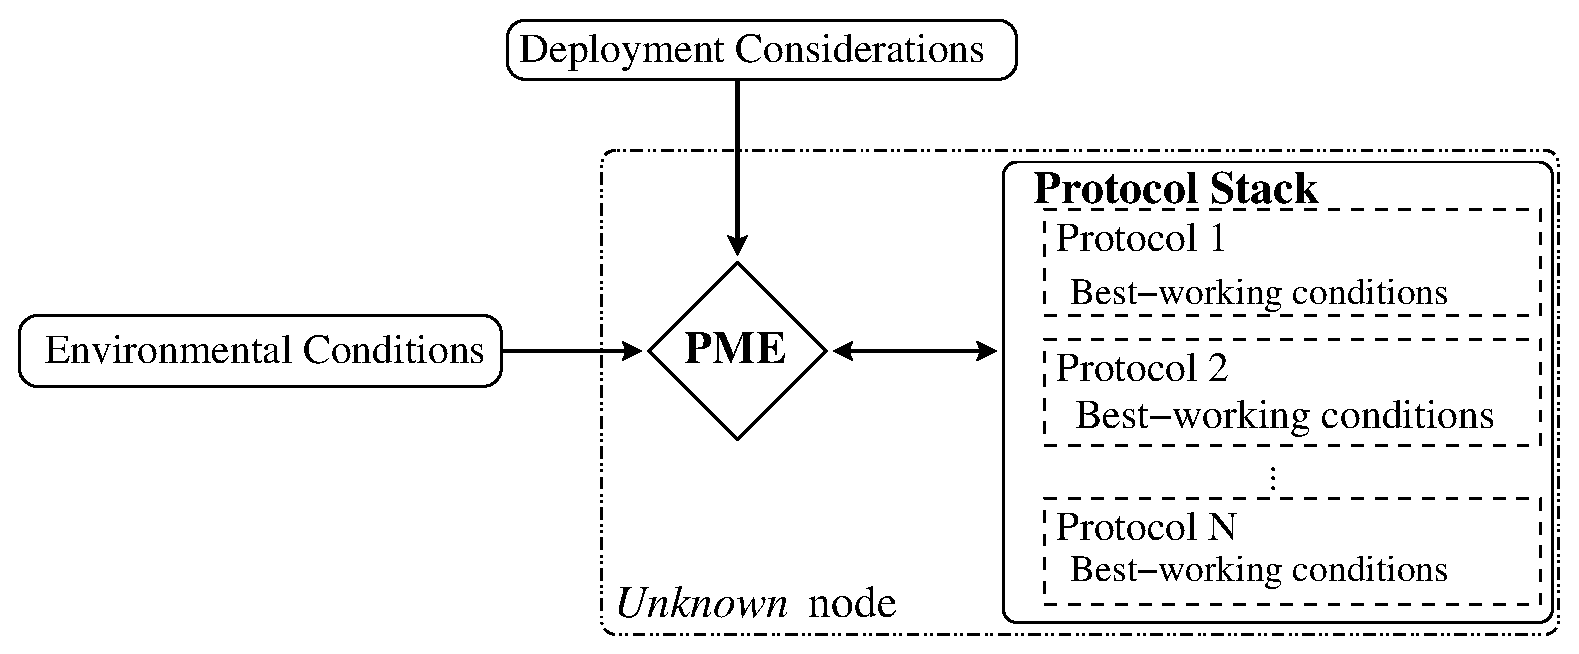
\includegraphics[width=0.83\linewidth]{section3/figures/LocProc_small.eps}
  \caption{Localization procedure: architecture
  \label{fig:LocProc}}
\end{figure*}

\subsection{Best-working environmental conditions}\label{bestWorkingConditions}
Some protocols perform better than others under different conditions. For instance, some \emph{Anchor}-based localization techniques (like the ones described in Section~\ref{literature}) require more connections to \emph{Anchors} than others~\cite{rang:loc:techniques}.

When referring to best-working environmental conditions, it is to point out network-environment metrics that would help a determined localization protocol to work more efficiently, like: number of effective connections of the type \emph{unknown-Anchor}, current delay, available bandwidth, network size or processing capabilities of the nodes.

Up-to-date information of the node's environmental conditions aids the process of determining which localization protocol is more capable of achieving the deployment considerations.

\subsection{Deployment considerations}\label{deploymentConsiderations}
Each deployment has defined goals and restrictions, like: long/coarse network lifetime, high/coarse accuracy, short/coarse localization traffic overhead or high/low localization protocol convergence time. These are tightly related to the application running over it.

Each localization protocol has its best-working environmental conditions, that when complied allow the protocol to provide satisfactory results and follow the deployment considerations.

\subsection{Pattern Matching Engine (PME)}\label{PME}
Is a module inside the localization procedure responsible for translating the \emph{unknown} node's environmental conditions into localization protocols than could comply with the deployment considerations. That is, for certain deployment considerations the PME will select a set of appropriate localization protocols where their best-working environmental conditions are met. If all the conditions are satisfied, the PME prioritizes the protocol that better complies with the deployment considerations. 

The architecture of the localization procedure is shown in Figure~\ref{fig:LocProc}, whence it can be appreciated the PME gathering environmental conditions and deployment considerations to select the appropriate localization protocols.

%shows an overview of the localization procedure's architecture and highlights the role of the PME.

\section{Evaluation} \label{simulation}
  This work considers two well-known distributed localization protocols for testing the proposed localization procedure: Lateration and Bounding-Box. Some of their differences are highlighted in Table~\ref{table:protocols}.

\begin{table}[tb]
  \centering
  \begin{threeparttable}[t]
    \caption{Localization Protocols' characteristics}
    \label{table:protocols}
    \begin{tabular}{c||c||c}
    \hline
    \bfseries Characteristic & \bfseries Lateration & \bfseries Bounding-Box\\
    \hline\hline 
    Env. Conditions & At least 4 \emph{Anchors} & At least 1 \emph{Anchor}\\
    Accuracy & 2-10 meters & Coarse\tnote{1}\\
    Energy Consumption & Low~\cite{laterationSpecs} & Very low\tnote{2}\\
    \hline
    \end{tabular}
    \begin{tablenotes}
    \item [1] Location area upper-bounded by \emph{Anchor}'s radio range (R).
    \item [2] Can be treated as a discrete problem.
    \end{tablenotes}
  \end{threeparttable}
\end{table}

In order to reveal the impact of the proposed localization procedure in terms of battery consumption, number of located nodes and localization error; a thousand simulations are performed per \emph{Anchor} density (from 10\% up to 100\% at 10\% increments) using a customized extension of the SENSE network simulator~\cite{sense}. The hardware and Medium Access (MAC) layer parameters implemented are presented in Table~\ref{tab:MAC_param}. Two propagation models are used: free space and a time-invariant and symmetrical shadowing model (from here on: Free space and Shadowing models respectively). The characteristics of the testing plane are highlighted in Table~\ref{tab:testingPlanes}. Nodes are randomly and uniformly distributed over the testing plane (as in Figure~\ref{fig:topology}) and the position estimation is based only on the received location information from Beacons. This is done to evaluate different \emph{Anchor} densities against a single \emph{unknown} node (i.e. 100\% \emph{Anchor} density means 
that a determined node will receive Beacons from all its neighbors and use the received location information to estimate its position, regardless if the recipient is an \emph{Anchor}).

To contrast the behavior of the localization procedure against the individual execution of the proposed localization protocols, the deployment considerations are set accordingly with the capabilities of the protocols (large network lifetime and coarse accuracy). The PME deterministically selects the appropriate protocols as it is explained in Section~\ref{PME}.

%The deployment considerations are set to require coarse network lifetime and coarse accuracy, which can be achieved with the tested localization protocols detailed in Table~\ref{table:protocols}. Also, the PME deterministically selects the appropriate localization protocol based only on the satisfaction of each of their best-working environmental conditions.

Results are shown with 99\% confidence intervals.

\begin{table}[tb]
  \begin{threeparttable}[t]
    \caption{Hardware and CSMA/CA Parameters}
    \label{tab:MAC_param}
    \begin{tabular}{c||c||c}
    \hline
    \bfseries Component & \bfseries Parameter & \bfseries Value\\
    \hline\hline 
    \multirow{8}{*}{Hardware} & Data rate & $19.2$~kbps\\ %1
			      & TX power & $0$~dBm\\ %2
			      & Reception threshold & $-148$~dBm\\ %3
			      & Carrier sense threshold & $-148$~dBm\\ %4
			      & Power consumption in TX mode & $24.75$~mW\\ %5
			      & Power consumption in RX/idle mode & $13.5$~mW\\ %6
			      & Power consumption in sleep mode & $15~\mu\rm{W}$\\ %7
			      %& Length of data field & $29$~bytes\\ %8
    \hline
    \multirow{4}{*}{CSMA/CA} & Headers & $11$~bytes\\ %1
			      & Beacon size & $40$~bytes\\ %2
			      & Contention window & $128$\\ %3
			      & Slot time & $417~\mu\rm{s}$\\ %4
    \hline
%     \multirow{1}{*}{Upper layers} & Network and Localization header & $150$~bits\\ %1
%     \hline
    \end{tabular}
  \end{threeparttable}
\end{table}

% The upper layer header shown in Table~\ref{tab:MAC_param} represents the data size of the Beacon packet, composed of the \emph{Anchor}'s position and other simulator-related parameters.

\begin{table}[tb]
  \centering
  \begin{threeparttable}[t]
  \caption{Characteristics of the testing plane based on~\cite{convexEstimation,fieldDimmensions}}
  \label{tab:testingPlanes}
  \begin{tabular}{c||c}
  \hline
  \bfseries Characteristic & \bfseries Value\\
  \hline\hline
  Area & $100\times100$~m$^{2}$\\
  Surface & Flat\\
  Distribution of nodes & Uniformly random\\
  \hline
  \end{tabular}
  \end{threeparttable} 
\end{table}

Each time a node connects with a new \emph{Anchor} (effectively receives its Beacons), the PME decides which localization protocol to execute. In the proposed simulation (and following Table~\ref{table:protocols}) if more than three \emph{Anchors} are connected to the \emph{unknown} node, then the PME will execute Lateration, otherwise Bounding-Box is selected. Further connections will lead the PME to reevaluate the node's situation and sequentially execute the appropriate localization protocol. As for Lateration, this can go on until six \emph{Anchors} are connected. Beyond this number, the accuracy refinements are not as significant to justify the penalty in battery consumption~\cite{beaconLimits}.

\begin{figure}[tb]
  \centering
  \includegraphics[width=0.7\linewidth, angle = -90]{section4/figures/topology.eps}
  \caption{Example random deployment of nodes
  \label{fig:topology}}
\end{figure}

\subsection{The effect of the tested channel models on the number of connection to \emph{Anchors}}\label{channel_considerations}
In Figure~\ref{fig:channelAndBeacons}, it is appreciated how the different propagation models affect the reception of Beacon packets; which in this evaluation is the sole environmental condition considered by the PME.

\begin{figure}[tb]
  \centering
  \includegraphics[width=0.7\linewidth, angle = -90]{section4/figures/avgBeaconPerNode.eps}
  \caption{Average number of \emph{Anchors} connected to each node}
  \label{fig:channelAndBeacons}
\end{figure}

Nodes in the Shadowing model are prone to more collisions than those in the Free space model. When there is high concentration of neighboring \emph{Anchors}, it is more probable that collisions occur. This results in a decreased number of \emph{Anchors} connected to each node, which has a direct impact on battery life, accuracy and number of located nodes.

\subsection{Individual execution of Lateration and Bounding-Box localization protocols}\label{individual_execution}
In order to better analyze the impact of the localization procedure on the network, metrics are gathered from the individual execution of the tested localization protocols.

These metrics reflect the protocols' impact on battery consumption, number of located nodes and the position estimation error.

\subsubsection{Battery consumption}\label{individual_battery_consumption}
apart from the battery consumption related with the normal operation of the nodes (listening the channel and Beacon reception), Lateration has an additional battery consumption associated with the execution of the algorithm (as mentioned in Section~\ref{lateration}). This seems to be increased in the Free space model because of the greater average number of \emph{Anchors} connected to each node (see Figure~\ref{fig:channelAndBeacons}~and~\ref{fig:battery}).

\begin{figure}[tb]
  \centering
  \includegraphics[width=0.7\linewidth, angle = -90]{section4/figures/battery.eps}
  \caption{Battery consumption of the individual execution of Lateration and Bounding-Box
  \label{fig:battery}}
\end{figure}

In the case of Bounding-Box, there is not additional battery consumption related to the execution of this algorithm. This is the reason why its added battery consumption is considered negligible when compared to Lateration.

%As for Bounding-Box, the algorithm seems to impose almost none additional battery consumption on the nodes. It is considered negligible compared to that of Lateration.

\subsubsection{Located nodes}
these are the nodes that successfully execute either of the localization protocols, resulting in a location estimation (see Figure~\ref{fig:locNodes}).

\begin{figure}[tb]
  \centering
  \includegraphics[width=0.7\linewidth, angle = -90]{section4/figures/locatedNodes.eps}
  \caption{Number of located nodes per tested localization protocol
  \label{fig:locNodes}}
\end{figure}

In the case of Lateration, at 30\% \emph{Anchor} density around 84\% and 95\% of the nodes get located in the Free space and Shadowing models respectively. Lower numbers are appreciated at 10-20\% \emph{Anchor} density due to the reduced/inexistent Beacons received at these densities.

Bounding-Box shows higher number of located nodes at 30\% \emph{Anchor} density (nearly 99\% in both propagation models) mainly due to a more coarse restriction for the execution of this protocol (only one Beacon).

\subsubsection{Error}
the proposed measure of error only considers nodes that were able to execute either of the localization protocols. It is defined as the straight line distance (in meters) between the node's estimated location and its real position (see Figure~\ref{fig:error}).

\begin{figure}[tb]
  \centering
  \includegraphics[width=0.7\linewidth, angle = -90]{section4/figures/error.eps}
  \caption{Straight line error from the estimated to the real node's position
  \label{fig:error}}
\end{figure}

The error in Lateration is related to inexact ranging measurements, which is greater in the Shadowing model given that for the calculations the node always assumes a Free space model. The location accuracy does not seem to improve significantly with the connection of more than six \emph{Anchors} without sacrificing battery life~\cite{beaconLimits}. Furthermore, it worsens with the degraded channel conditions imposed by the Shadowing propagation model.

For Bounding-Box, the Shadowing model reduces the average number of \emph{Anchors} received at the \emph{unknown} node, which translates in the elimination of some of the constraints that allow this protocol to increase its accuracy.

%For Bounding Box, the Shadowing model shows that there are \emph{Anchors} at more than R (R = simulated radio range calculated in free space) meters from the \emph{unknown} node that are also considered in the calculation, thus increasing the size of the location area estimated by the algorithm. 

\subsection{Localization procedure execution}\label{locProc_executions}
As mentioned in Section~\ref{PME}, PME will pick a localization protocol that given the node's environmental conditions, could comply with the deployment considerations.

\subsubsection{Battery consumption}
the difference between the battery consumption associated with the proposed localization procedure and that of Lateration is very small. For this reason they are considered similar (see Figure~\ref{pme:battery}).

\begin{figure}[tb]
  \centering
  \includegraphics[width=0.7\linewidth, angle = -90]{section4/figures/pmeBat.eps}
  \caption{Localization procedure's associated battery consumption when compared with Lateration
  \label{pme:battery}}
\end{figure}

Bounding-Box adds negligible battery consumption (as mentioned in Section~\ref{individual_battery_consumption}), therefore it is not included in Figure~\ref{pme:battery}, which only attempts to compare the average battery consumption of the individual execution of Lateration and the amount consumed by the proposed localization procedure.

\subsubsection{Located nodes}\label{locProc_locatedNodes}
the sum of located nodes (either with Lateration or Bounding-Box) reaches 99\% at \emph{Anchor} densities around 30\% (see Figure~\ref{pme:locNodes}).

\begin{figure}[tb]
  \centering
  \includegraphics[width=0.7\linewidth, angle = -90]{section4/figures/pmeLocNodes.eps}
  \caption{Located nodes with the proposed localization procedure
  \label{pme:locNodes}}
\end{figure}

With Free space model 100\% localization is achieved at 20\% \emph{Anchor} density. On the other hand, in the Shadowing model 100\% localization is achieved at slightly higher densities, on average around 40\%.

The number of located nodes with the proposed localization procedure exceeds those of Lateration, in fact Figure~\ref{pme:locNodes} looks more like the curves of Bounding-Box in Figure~\ref{fig:locNodes}.

\subsubsection{Error}
This measure illustrates the average distance in meters between each node's estimated location and its real position. The prefix \emph{Loc. Proc.} in Figure~\ref{pme:error} highlights the fact that these are results gathered from the execution of the localization procedure.

\begin{figure}[tb]
  \centering
  \includegraphics[width=0.7\linewidth, angle = -90]{section4/figures/pmeAverageErrorPerProtocol.eps}
  \caption{Associated error after protocol selection
  \label{pme:error}}
\end{figure}

Figure~\ref{pme:error} displays the average error for each type of channel model. It also considers the number of nodes executing either Lateration or Bounding-Box. So the average error is expressed as: $Avg_{A}^{ch} = (E_{L}~n_{L} + E_{BB}~n_{BB}) /n_{L}+n_{BB}$. Where $Avg_{A}^{ch}$ is the average error with a $ch$ channel model and $A$ \emph{Anchor} density. $n_{L}$ are the number of nodes executing Lateration while $n_{BB}$ are the same but in the case of Bounding-Box. $E_{L}$ and $E_{BB}$ refer to the average line error for nodes executing Lateration and Bounding-Box respectively.

Due to increased ranging measurement errors, the estimation in the Shadowing model presents more erroneous estimations than the Free space model, as in Figure~\ref{fig:error}. Although at $30$\% \emph{Anchor} density the localization procedure incurs in greater average error as compared with the individual execution of Lateration, it manages to increase the average number of located nodes. This is significantly important, given that without the localization procedure many nodes were to be left without a location estimation, or what it is the same as having an undetermined measure of error.

A carefully selected set of localization protocols working with different ranges of environmental conditions, ensures that most of the nodes in the deployment get located. In the testings presented in this section, Bounding-Box is the responsible for locating the most isolated nodes, while Lateration focuses on accuracy. Selecting and characterizing more accurate protocols will reduce the errors and maintain the high number of located nodes that the localization procedure achieves. All of this while preserving the levels of battery consumption similar to the individual execution of the selected protocols.

\section{Conclusions} \label{conclusions}
  %In order to improve the simulation's results, more accurate ranging techniques need to be used to leverage the high levels of errors provided by RSSI ranging technique. As for the range-free protocol used, its performance can be enhanced by incorporating ranging measurements in order to add constraints to the underlying optimization problem (as in~\cite{convexEstimation}). These measures will result in an overall reduction of the error.

%The presented localization procedure considers the \emph{unknown} nodes' environmental conditions in order to make a more intelligent protocol selection. Coupled with the deployment considerations, nodes avoid incurring in additional battery consumption related to simultaneous protocol execution (as it is the case in~\cite{composability}), given that the PME selects a single protocol each time.

%In the simulation, by correctly identifying the best-working environmental conditions of each protocol the localization procedure is able to locate more nodes than by their individual execution. Also, the localization procedure effectively locates 100\% of the nodes in the deployment at \emph{Anchor} densities around $20$\% in a free space model, while the individual execution of the tested range-based localization protocol achieves the same at around $40$\%.

%Apart from the specific enhancements suggested for each protocol implementation, upon localization a newly located node may broadcast its estimated location so other \emph{unknown} nodes may enrich their environmental conditions. This location information exchange by newly located nodes introduces new challenges related to listening time and error propagation \cite{alsindi2006error}. Given that with this new approach the \emph{unknown} nodes would not only listen to \emph{Anchors} but also to other located nodes, the overall energy consumption would be increased.

%Exchanging the environmental conditions of each node opens the door for more complex and centralized localization algorithms \cite{pal2010localization,alippi2006rssi}. This requires specifics on how the \emph{unknown} node should identify the conditions where a centralized localization protocol is better for the given deployment considerations, what are the favorable environmental conditions and how these can be matched into deployment considerations.

In this work a new and flexible approach to the localization problem in randomly-deployed WSNs is presented. It extends the proposal of~\cite{composability}, which considers the composability of localization protocols as a robust solution. 

The localization procedure incorporates flexibility on the selection of localization protocols by determining which is more capable of achieving predetermined deployment considerations under the environmental conditions surrounding each \emph{unknown} node. 

It is designed to admit several localization protocols, definitions of environmental conditions and deployment considerations; which makes it a good choice for random deployments, like~\cite{airDroppedVolvano}.

A set of evaluations were preformed with two well-know localization protocols, referred to as Lateration (range-based) and Bounding-Box (range-free). Results show that the localization procedure is able to locate more nodes than by their individual execution, suggesting a more intelligent and flexible localization scheme that considers the current state of the nodes before making decisions about its future state.

% Also, the localization procedure effectively locates 100\% of the nodes in the deployment at \emph{Anchor} densities around $20$\% in a free space model, while the individual execution of the tested range-based localization protocol achieves the same at around $40$\%.

In order to improve the current proposal, it is important to identify the environment metrics that correlate with the performance of each localization protocol to be used. Once understood, simple adjustments in the PME would enable it to comply with the deployment considerations in a more effective way. Moreover, the PME can be adapted to make a protocol selection based not only on its own, but also with the surrounding nodes' environmental conditions. This opens the door to more complex and centralized localization algorithms, like~\cite{pal2010localization}~and~\cite{alippi2006rssi}.
  
\bibliographystyle{Classes/IEEEtran}
\bibliography{IEEEabrv,ref}
  
\end{document}

